\section{Linear Systems}

Linear equations appear in a variety of practical contexts, such as economics, social sciences, and data science. Very often, linear equations come in groups. For example, the supply and demand curves for a good are often treated as linear functions and we want to consider both equations at the same time, instead of considering them separately.

\begin{colourframe}[tolGrey]{\bf Big Questions}
	
	\begin{itemize}
		\item What are linear equations and linear systems?
		\item What is a solution to a linear system and how can we verify if a point is a solution?
		\item How can linear systems appear in the real world?
	\end{itemize}
\end{colourframe}


\subsection*{Linear Equations}

\begin{example}\label{ex:intersection}

	The number of cars entering and leaving an intersection is recorded for several months. The diagram below gives the average number of cars entering and leaving the intersection in each direction per hour. What can we say about the net number of cars entering and leaving the intersection from the south and east, which we will call $x$ and $y$ respectively?
	
		\begin{center}
			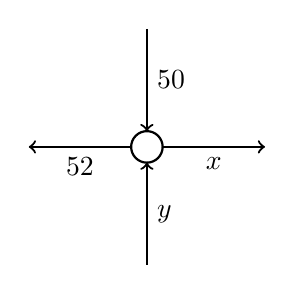
\begin{tikzpicture}
				\draw[thick] (0,0) circle (0.2);
				\draw[thick, ->] (0,1.5) -- (0,0.2) node[right, midway]{$50$};
				\draw[thick, ->] (0.2,0) -- (1.5,0) node[below, midway]{$x$};
				\draw[thick, <-] (0,-0.2) -- (0,-1.5) node[right, midway]{$y$};
				\draw[thick, <-] (-1.5,0) -- (-0.2,0) node[below, midway]{$52$};
			\end{tikzpicture}
		\end{center}
		
	At an intersection, the number of cars entering and leaving must be equal. We can use this to derive an equation:
	\begin{align*}
		\text{Cars In} &= \text{Cars Out}\\
		50 + y &= 52+x
	\end{align*}
	
	We usually group variables together and constants together. In tbis case, we would typically rewrite this equation describing the traffic as $x - y = -2.$

	This tells us that any configuration of traffic where $x - y = -2$ is a possible traffic flow for this intersection. For example, we could have 10 cars leaving the intersection heading east and 12 cars entering from the south every hour, so $x = 10$ and $y = 12$. We can visualize the collection of all possible traffic configurations by graphing this equation. 
	
	\begin{center}
		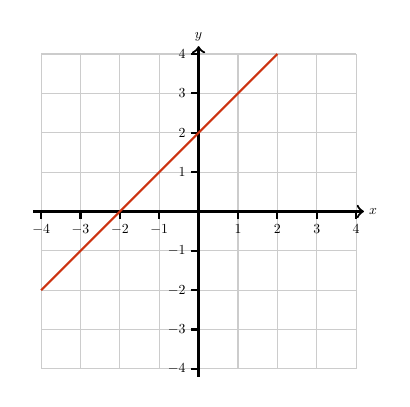
\begin{tikzpicture}[scale = 0.5]
			\draw[black!20] (-4,-4) grid (4,4);
			\draw[thick, ->] (-4.2,0) -- (4.2,0) node[right, scale = 0.5]{$x$};
			\draw[thick, ->] (0,-4.2) -- (0,4.2) node[above, scale = 0.5]{$y$};
			
			\foreach \x in {-4,-3,-2,-1,1,2,3,4}{
				
				\draw[thick] (\x,0) -- (\x,-0.2) node[below, scale = 0.5]{$\x$};
			}
			
			\foreach \y in {-4,-3,-2,-1,1,2,3,4}{
				
				\draw[thick] (0,\y) -- (-0.2,\y) node[left, scale = 0.5]{$\y$};
			}
			\definecolor{tolRed}{HTML}{CC3311} 
			\draw[thick, color = tolRed] (-4,-2) -- (2,4);
		\end{tikzpicture}
	\end{center}

\end{example}

\begin{example}\label{ex:supdem}
	The demand and supply of a good are given by the equations
	\begin{align*}
		{\color{tolRed}\text{Demand}} &= {\color{tolRed}6 - 3p}\\
		{\color{tolBlue}\text{Supply}} &= {\color{tolBlue}2p - 4}
	\end{align*}
	
	As consumers and the supplier react to changes in the amount purchased and the price the good is sold for, the price and quantity will tend towards a market equilibrium where demand and supply are equal. At this equilibrium, we will have $\text{demand} = \text{supply} = q$, which gives us the system of equations
	\begin{align*}
		{\color{tolRed}q} &= {\color{tolRed}6 - 2p}\\
		{\color{tolBlue}q} &= {\color{tolBlue}2p - 4}.
	\end{align*}
	
	Note that we can solve this system to find the equilibrium price is $p = 2.5$ and the equilibrium quantity is $q = 1$. To see that this is actually a solution, we can substitute $p = 2.5$ and $q = 1$ into the equations to verify that they are true. We can also find this equilibrium point by graphing the equations.

	\begin{center}
		\begin{tikzpicture}[scale = 0.5]
			\draw[black!20] (0,0) grid (6,6);
			\draw[thick, ->] (0,0) -- (6.2,0) node[right, scale = 0.5]{$p$};
			\draw[thick, ->] (0,0) -- (0,6.2) node[above, scale = 0.5]{$q$};
			
			\foreach \x in {1,...,6}{
				
				\draw[thick] (\x,0) -- (\x,-0.2) node[below, scale = 0.5]{$\x$};
			}
			
			\foreach \y in {1,...,6}{
				
				\draw[thick] (0,\y) -- (-0.2,\y) node[left, scale = 0.5]{$\y$};
			}

			\draw[thick, color = tolRed] (0,6) -- (3,0);
			\draw[thick, color = tolBlue] (2,0) -- (5,6);

			\filldraw (2.5,1) circle (2pt) node[right, scale  = 0.7]{$(2.5,1)$};

		\end{tikzpicture}
	\end{center}
	
	Notice that the equilibrium point $p = 2.5$ and $q = 1$ corresponds to the intersection of the supply and demand curves. That is, it is the only point which is on both lines.

\end{example}

These examples involved equations of a very simple form. We saw by graphing them that the equations gives us lines. As such, we call them \textit{linear equations.}

\begin{definition}
	A \textbf{linear equation} is any equation which can be written as
	
	$$a_1x_1 + a_2x_2 + \dots + a_nx_n = b$$
	
	\noindent where $x_1,\dots, x_n$ are variables and $a_1,\dots, a_n, b$ are constants.
\end{definition}

\begin{example} 

	The equations in the previous two examples, $x - y = -2$, $q = 6-2p$, and $q = 2p - 4$ are all examples of linear equations. In applications, it is very common for the variables in your linear system to be represented by symbols other than $x_1, \dots, x_n$.

\end{example}

\begin{example}
	%This example assumes that the students have seen linear functions from \R^2 to \R already.
	Consider the linear equation
	
	$$2x - 3y + z = 4.$$
	
	Graphically, this equation defines a plane in 3-dimensional space. We can see this by rearranging the equation as
	
	$$z = 4 - 2x + 3y.$$
	
	\noindent This equation gives the graph of the function $f(x,y) = 4 - 2x +3y$, which is a linear function. As we have seen previously, the graph of a linear function of two variables is a plane.
\end{example}



\subsection*{Systems of Linear Equations and their Solutions}

In the supply and demand example above, we saw that linear equations can appear together and that the intersection of the corresponding lines had a natural interpretation. It is very common to have a collection of linear equations in the same variables and to care about points that satisfy all of those equations.

\begin{definition}
	Any set of linear equations is called a \textbf{linear system} or a \textbf{system of linear equations.}
\end{definition}


\begin{example}\label{ex:twoplanes}

	The system of linear equations 
	\[
	\arraycolsep=1.4pt
	\begin{array}{rcrcrl}
		{\color{tolRed}x} & {\color{tolRed}+} & {\color{tolRed}y}& {\color{tolRed}-} & {\color{tolRed}2z} &= {\color{tolRed}0}\\
		{\color{tolBlue}x} &{\color{tolBlue}-}& {\color{tolBlue}2y} &{\color{tolBlue}-} & {\color{tolBlue}3z} &= {\color{tolBlue}-9}
	\end{array}
	\]

	\noindent can be visualized by the following graph.

	\begin{center}
		\tdplotsetmaincoords{70}{110}
		\begin{tikzpicture}[tdplot_main_coords, scale = 0.7]
			\tikzstyle{plane1top} = [very thick, opacity = 1, fill = tolRed];
			\tikzstyle{plane1bot} = [very thick, opacity = 0.7, fill = tolRed];
			\tikzstyle{plane2} = [very thick, opacity = 0.7, fill = tolBlue];
			\tikzstyle{axis} = [very thick, black, ->]
			\tikzstyle{grid} = [thin, black!20]

			\foreach \x in {1,2,3,4,5}{
				\draw (\x,0,0) -- (\x,5,0);	
				\draw (\x,0,0) node[anchor = south east, scale = 0.7]{$\x$};			
			}

			\foreach \y in {1,2,3,4,5}{
				\draw (0,\y,0) -- (5,\y,0);
			}

			\foreach \y in {1,5}{
				\draw (0,\y,0) node[anchor = south, scale = 0.7]{$\y$};
			}
			
			\foreach \z in {1,2,3,4}{
				\draw (0,0,\z) -- (0.05,-0.2,\z);
			}

			\draw[thick] (0,0,4) -- (0.05,-0.2,4) node[anchor = east, scale = 0.7]{$4$};
			
			\draw[axis] (0,0,0) -- (5.4,0,0) node[anchor = north, scale = 0.7]{$x$};
			\draw[axis] (0,0,0) -- (0,5.2,0) node[anchor = west, scale = 0.7]{$y$};
			\draw[axis] (0,0,0) -- (0,0,4.2) node[anchor = south, scale = 0.7]{$z$};

			%\draw (0,0,0) grid (5,5,0);
			\draw[plane1bot] (0,0,0) -- (5,0, 2.5) -- (5,5,5) -- (0,5,2.5) -- cycle;
			\draw[plane2] (0,0,3) -- (5,0,4.666) -- (5,5,1.333) -- (0,5,-0.333) -- cycle;
			\draw[plane1top] (0,{18/7},{9/7}) -- (0,5,2.5) -- (5,5,5) -- (5,{13/7}, {24/7}) -- cycle;
			
		\end{tikzpicture}
	\end{center}
	
	The red plane corresponds to all points satisfying the equation $x+y - 2z = 0$ and the blue plane corresponds to all points satisfying the equation $x - 2y - 3z = -9$. The set of all points satisfying both equations corresponds to the intersection of the planes, since if a point satisfies both equations then it must be on both planes. Notice that their intersection is a line. If you want to see the graph of this system of equations from a different perspective, you can find another visualization at this link to {\color{tolRed}\href{https://www.math3d.org/F9anqa662}{Math3D.}}

\end{example}

\begin{definition}
	A \textbf{solution} to a system of linear equations
	\[
	\arraycolsep=1.4pt
	\begin{array}{rcrcccrl}
		a_{11} x_1 &+& a_{12}x_2& +& \dots &+& a_{1n}x_n 	&= b_1\\
		a_{21} x_1 &+& a_{22}x_2& +& \dots &+& a_{2n}x_n 	&= b_2\\
				&	&		&	& \vdots &	&	&	\\
		a_{m1}x_1& +& a_{m2}x_2 &+& \dots &+& a_{mn}x_m &= b_m
	\end{array}
	\]
	
	\noindent is a point $(s_1,\dots, s_n)$ with $s_1,\dots,s_n$ constant such that taking $(x_1,\dots,x_n) = (s_1,\dots,s_n)$ satisfies each equation in the system. I.e., $a_{k1}s_1 + a_{k2}s_2 + \dots + a_{kn}s_n = b_k$ is true for $k = 1, 2, \dots, m$.
	
	The set of all solutions of a system is called its \textbf{solution space}.
\end{definition}

\begin{example}
	Recall that the supply and demand system
	\begin{align*}
		q &= 6-2p\\
		q &= 2p-4
	\end{align*}
	
	\noindent is satisfied when $p = 2.5$ and $q = 1$. Therefore, the equilibrium point $(p,q) = (2.5,1)$ is a solution to this system. From the graph in example \ref{ex:supdem}, we recognize that this solution corresponds to the intersection of the two lines $q = 6-2p$ and $q = 2p-4$. We can also see from the graph that this is the only solution. Therefore, the solution space of this system is a single point.
\end{example}

\begin{example}
	In example \ref{ex:twoplanes}, we saw that the set of points satisfying both of the equations 
	\[
	\arraycolsep=1.4pt
	\begin{array}{rcrcrl}
		x  &+& y &-& 2z &= 0\\
		x &-& 2y &-& 3z &= -9
	\end{array}
	\]
	
	\noindent is a line. However, we cannot use the graph to easily verify if a point is a solution or to give a formula for all of the solutions of this system.
	
	Is $(1,1,1)$ a solution to this system? To check, we can substitute $(x,y,z) = (1,1,1)$ into the system to see if the resulting equations are true. Doing so yields:
	\begin{align*}
		1 + 1 - 2(1) &= 0\\
		1 - 2(1) - 3(1) = -4 &\ne -9
	\end{align*}
	
	Therefore, $(1,1,1)$ is not a solution to this system of equations.

\end{example}

We've seen that the solution space for a linear system can be a single point. However, this is not the only possibility for a solution space. Let's investigate the geometry of solution spaces in two and three dimensions.


\begin{example}
	For a system of linear equations in two variables
	\[
	\arraycolsep=1.4pt
	\begin{array}{rcrl}
		a_{11}x &+& a_{12}y &= b_1\\
		a_{21}x &+& a_{22}y &= b_2
	\end{array}
	\]
	
	\noindent the solution space is all points $(x,y)$ satisfying \textbf{both} equations. What could the solution space of this system look like? 
	
	Note that both of these equations describe lines. Let $L_1$ be the line $a_{11}x + a_{12}y = b_1$ and $L_2$ be the line $a_{21}x + a_{22}y = b_2$. Consider the following graphs.
	
	\begin{center}
		
		\raisebox{-0pt}{
			\begin{minipage}{0.3\textwidth}
				\begin{center}
					\begin{tikzpicture}[scale = 0.6]
						\draw[thin, black!20] (-2,-2) grid (2,2);
						\draw[thick, ->] (-2.2, 0) -- (2.2,0) node[right, scale = 0.6]{$x$};
						\draw[thick, ->] (0,-2.2) -- (0,2.2) node[right, scale = 0.6]{$y$};
						
						\foreach \x in {-2,-1,1,2}{
							\draw (\x,0) -- (\x,-0.1) node[below, scale = 0.6]{$\x$};
						}
						\foreach \y in {-2,-1,1,2}{
							\draw (0,\y) -- (-0.1,\y) node[left, scale = 0.6]{$\y$};
						}
						
						\draw[thick, color = tolRed] (-2,0) -- (2, 1.3333)node[anchor = west, scale = 0.6]{$L_1$};
						\draw[thick, color = tolBlue] (0,-2) -- (1.3333,2)node[anchor = south, scale = 0.6]{$L_2$};
					
					\end{tikzpicture}\\
					{\scriptsize Graph A}
				\end{center}
			\end{minipage}
		}
		\raisebox{-0pt}{
			\begin{minipage}{0.3\textwidth}
				\begin{center}
					\begin{tikzpicture}[scale = 0.6]
						\draw[thin, black!20] (-2,-2) grid (2,2);
						\draw[thick, ->] (-2.2, 0) -- (2.2,0) node[right, scale = 0.6]{$x$};
						\draw[thick, ->] (0,-2.2) -- (0,2.2) node[right, scale = 0.6]{$y$};
						
						\foreach \x in {-2,-1,1,2}{
							\draw (\x,0) -- (\x,-0.1) node[below, scale = 0.6]{$\x$};
						}
						\foreach \y in {-2,-1,1,2}{
							\draw (0,\y) -- (-0.1,\y) node[left, scale = 0.6]{$\y$};
						}
			
						\draw[thick, color = tolRed] (-1.5,-2) -- (-1.5, 2)node[anchor = south, scale = 0.6]{$L_1$};
						\draw[thick, color = tolBlue] (0.7,-2) -- (0.7,2)node[anchor = south, scale = 0.6]{$L_2$};
					
					\end{tikzpicture}\\
					{\scriptsize Graph B}
				\end{center}
			\end{minipage}
		}
		\raisebox{-3pt}{
			\begin{minipage}{0.3\textwidth}
				\begin{center}
					\begin{tikzpicture}[scale = 0.6]
						\draw[thin, black!20] (-2,-2) grid (2,2);
						\draw[thick, ->] (-2.2, 0) -- (2.2,0) node[right, scale = 0.6]{$x$};
						\draw[thick, ->] (0,-2.2) -- (0,2.2) node[right, scale = 0.6]{$y$};
						
						\foreach \x in {-2,-1,1,2}{
							\draw (\x,0) -- (\x,-0.1) node[below, scale = 0.6]{$\x$};
						}
						\foreach \y in {-2,-1,1,2}{
							\draw (0,\y) -- (-0.1,\y) node[left, scale = 0.6]{$\y$};
						}
						
						\draw[very thick, color = tolBlue] (-2,-2) -- (2,2)node[anchor = south west, scale = 0.6]{$L_2$};		
						\draw[color = tolRed] (2,2) -- (-2, -2)node[anchor = north east, scale = 0.6]{$L_1$};
					\end{tikzpicture}\\
					\raisebox{7.3pt}{\scriptsize Graph C}
				\end{center}
			\end{minipage}
		}
	\end{center}
	
	In graph A, we have a typical example of two non-parallel lines. Two non-parallel lines must intersect at a single point. Therefore, if the linear system corresponds to two non-parallel lines, the solution space will be a point.
	
	If the two lines given by the linear system are parallel, there are two situations that can occur. First, we could have two different lines which are parallel. Such lines would never intersect, as depicted in graph B. As such, the system would have no solutions. Alternatively, the two lines could be the same line. In that case, any point on one of the lines would be on both lines and therefore a solution, as depicted in graph C. If the two lines are identical, there would be infinitely many solutions. 

\end{example}

This example suggests that several different things can happen. A linear system can have exactly one solution, it can have infinitely many solutions, or it can have no solutions.

\begin{definition}
	A linear system is \textbf{consistent} if it has at least one solution. A linear system with no solutions is called \textbf{inconsistent}.
\end{definition}

It is not convenient to have to graph a linear system each time we want to find its solutions or to determine if it is consistent or inconsistent. We shall see shortly that there is an algebraic process that will allow us to solve any linear system.

\begin{exercise}
	What can the solution space for a system of three linear equations in three variables
	\[
	\arraycolsep=1.4pt
	\begin{array}{rcrcrl}
		a_{11}x &+& a_{12}y &+& a_{13}z &= b_1\\
		a_{21}x &+& a_{22}y &+& a_{23}z &= b_2\\
		a_{31}x &+& a_{32}y &+& a_{33}z &= b_3		
	\end{array}
	\]
	
	\noindent look like? For each possible solution space, sketch a picture of three planes that illustrates that solution space. Can you find more than one way to draw your picture that results in the same solution space? In each case, explain whether the system is consistent or inconsistent. If it is consistent, how many solutions does it have?
\end{exercise}

\vfill











